\documentclass{beamer}

\usetheme{Copenhagen}
\usecolortheme{beaver}
\usefonttheme[onlymath]{serif}

\usepackage[utf8]{inputenc}
\usepackage{graphicx,array,kotex,verbatim,multirow}
\author{김선중}
\date{\today}

%% toc for each section
\AtBeginSection[]
{
 \begin{frame}<beamer>
 \frametitle{}
 \tableofcontents[currentsection,hideallsubsections]
 \end{frame}	
}

%% example environment
\newcounter{chap}
\newcounter{ex}
\makeatletter
\def\th@mystyle{%
    \normalfont % body font
    \setbeamercolor{block title example}{bg=orange,fg=white}
    \setbeamercolor{block body example}{bg=orange!20,fg=black}
    \def\inserttheoremblockenv{exampleblock}
  }
\makeatother
\theoremstyle{mystyle}
\newtheorem*{exam}{\refstepcounter{ex}Example \thechap-\theex}

\newcommand{\pb}[1]%\Phantom + fBox
{\fbox{\phantom{\ensuremath{#1}}}}

\newcommand{\att}{\ensuremath{\text{attn}}}
\newcommand{\sof}{\ensuremath{\text{softmax}}}	

\usepackage{listings,color}
\definecolor{dkgreen}{rgb}{0,0.6,0}
\definecolor{gray}{rgb}{0.5,0.5,0.5}
\definecolor{mauve}{rgb}{0.58,0,0.82}
\lstset{frame=tb,
  language=Python,
  aboveskip=3mm,
  belowskip=3mm,
  showstringspaces=false,
  columns=flexible,
  basicstyle={\small\ttfamily},
  numbers=none,
  numberstyle=\tiny\color{gray},
  keywordstyle=\color{blue},
  commentstyle=\color{dkgreen},
  stringstyle=\color{mauve},
  breaklines=true,
  breakatwhitespace=true,
  tabsize=3
}


\title{Elementary Bayesian Optimization}

\setcounter{chap}{2}

\begin{document}
%
\frame{\titlepage}

%
\begin{frame}
\frametitle{Table of Contents}
\begin{enumerate}[1.]
\item
References
\item
Brief History of Bayesian Optimzation
\item
An Overview of Bayesian Optimizaiton
\item
A Few Elements of Bayesian Optimization
\begin{enumerate}
\item
Priors
\item
Covariance Function
\item
Acquisition function
\end{enumerate}
\end{enumerate}
\end{frame}

%%%
\section{References}

%
\begin{frame}
\frametitle{References}
\begin{enumerate}
%\item[4.]
%Jonas Močkus, 1975, ``On the Bayes Methods for Seeking the Extremal Point''
\item[1.]
James Bergestra, et al., 2011, ``Algorithms for Hyper-Parameter Optimzation''
\item[2.]
Jasper Snoek, et al., 2012, ``Practical Bayesian Optimization of Machine Learning Algorithms''
\end{enumerate}
\end{frame}

%
\begin{frame}{References : Keywords in [1] and [2]}
\begin{itemize}
\item
Gaussian Process(GP)
\item
Expected Improvement(EI)
\item
Sequential Model Based Global Optimization(SMBO)
\item
Deep Belief Network (DBN)
\item
Tree-structured Parzen Estimator Approach(TPE)
\end{itemize}
\end{frame}

%
\begin{frame}
\frametitle{References}
\begin{enumerate}
\item[3.]
Peter I. Frazier, 2018, ``A Tutorial on Bayesian Optimization''
\item[4.]
Peter I. Frazier, ``TutORial : Bayesian Optimization'', \url{www.youtube.com/watch?v=c4KKvyWW_Xk&t=1924s}
\item[5.]
Eric Brochu, et al., 2010, TR-2009 ``A Tutorial on Bayesian Optimization of Expensive Cost Functions, with Application to Active User Modeling and Hierarchical Reinforcement Learning''
\end{enumerate}
\end{frame}

%%
\section{Brief History of Bayesian Optimzation[3, 5]}

%
\begin{frame}{Brief History of Bayesian Optimzation}
(Section 1 in [3], Section 2.5 in [5])\\[20pt]
Bayesian optimization is originated with the work of \alert{Kushner}, \alert{Žilinskas} and \alert{Mockus}.
\begin{itemize}
\item
(Kushner, 1964) extended the method of sampling in finding maximum of a function.
He extended to a new method of considering multiple sampling, which is proved to be useful than the former ones.
\item
In the paper (Žilinskas, 1975), the one-stage Bayesian method for one-variable minimzation (OBM) is suggested.
\end{itemize}
\end{frame}

%
\begin{frame}{Brief History of Bayesian Optimzation}
\begin{itemize}
\item
(Močkus, 1978) together with Žilinskas et al, applied Bayesian approach to the problem of finding global maximum of multiextremal functions.
\item
(Močkus, 1975) also investigated Bayesian optimzation of multiextremal functions.
\item
These methodology is presented in his book ``Bayesian Approach to Global Optimization'' (Močkus, 1989).
\end{itemize}
\end{frame}

%
\begin{frame}{Brief History of Bayesian Optimzation}
Bayesian optimization received substantially more attention and popularized by Jones et al.
\begin{itemize}
\item
In (Jones, 1998), he adopted response surface which is often called \alert{surrogate function}, to reduce time and cost to approximate the given function.
The mechanism is called \alert{efficient global optimization}(EGO) algorithm.
%Since the advent of EGO, many innovations are developed in that same literature
\item
EGO is applied to derivative-free optimization and experimental design[5].
\end{itemize}
\end{frame}

%
\begin{frame}{Brief History of Bayesian Optimzation}
Following (Jones, 1998), innovations developed in that same literature includes
\begin{itemize}
\item
multi-fidelity optimization (Huang, 2006; Sóbester, 2004)
\item
multi-objective optimization (Keane, 2006; Knowles, 2006; Močkus; Močkus, 1991)
\item
study of convergence rates(Calvin,1997; Calvin and Žilinskas, 2000; Calvin and Žilinskas, 2005; Calvin and Žilinskas, 1999)
\end{itemize}
\end{frame}

%
\begin{frame}{Brief History of Bayesian Optimzation}
The observation made by (Snoek, 2012) that BayesOpt is useful for training deep neural networks sparked a surge of interest within machine learning.
\begin{itemize}
\item
multi-task optimization (Swersky, 2013; Toscano-Palmerin and Frazier, 2018)
\item
multi-fidelity optimization for DNN (Klein et al., 2016),
\item
parallel methods (Ginsbourger, 2007, 2010; Wang, 2016a; Wu and Frazier, 2016)
\item
Gaussian process regression (Kleinjnel, 2008 ; Salemi, 2014 ; Mehdad and Kleijnen, 2018)
\end{itemize}
\end{frame}

%%%
\section{An Overview of Bayesian Optimizaiton[3, 5]}

%%
\subsection{An Overview of Bayesian Optimizaiton}
\begin{frame}{An Overview of Bayesian Optimizaiton}
\begin{itemize}
\item
Bayesian optimization is a method for maximizing (or minimizing) a function \(f:A\to\mathbb R\) where \(A\subset\mathbb R^d\).
Sometimes we write
\[\max_{x\in A}f(x).\]
\item
The \alert{objective function} \(f\) is unknown, we are to sample from the domain \(A\) using \alert{surrogate function} and \alert{acquisition function} to achieve our goal.
\end{itemize}
\end{frame}

%
\begin{frame}{An Overview of Bayesian Optimizaiton}
In our problem, we are assuming the followings;
\begin{itemize}
\item
\(d\), the dimension of the domain, is assumed to be less than 20.
\item
\(x\), the independent variable, is assumed to be within a simple domain \(A\) like \(k\)-cube \(\prod_{i=1}^k[a_i,b_i]\).
\item
\(f\) is assumed to be a good function in a sense that it is (Lipschitz) continuous.
But it is not differentiable.
So it is impossible to approximate \(f\) using its derivatives or its second derivatives.
\item
Still, \(f\) is really complicated function, so one can not evaluate the value in low cost.
And it lacks special structure like concavity or linearity.
\end{itemize}
\end{frame}

%
\begin{frame}{Overview of Bayesian Optimization}
\begin{itemize}
\item
It is called \emph{Bayesian} because it uses the famous ``Bayes theorem''
\[P(M|E)\propto P(E|M)P(M).\]
\item
The \alert{posterior} probability of a model \(M\) given \alert{evidence} \(E\) is proportional to the \alert{likelihood} of \(E\) given \(M\), multiplied by the \alert{prior} probability of M.
\item
Let \(x_i\) be the \(i\)th sample.
Consider the set
\[D_{1:t}=\left\{\left(x_i,f(x_i)\right)|1\le i\le t\right\}\]
of ordered pair \((x_i,f(x_i)\), which plays a role of evidence.
% and call \(f(x_i)\) by the observation of \(x_i\).
We have
\[P(f|D_{1:t})\propto P(D_{1:t}|f)P(f).\]
\end{itemize}
\end{frame}

%
\begin{frame}{Overview of Bayesian Optimization}
\begin{center}
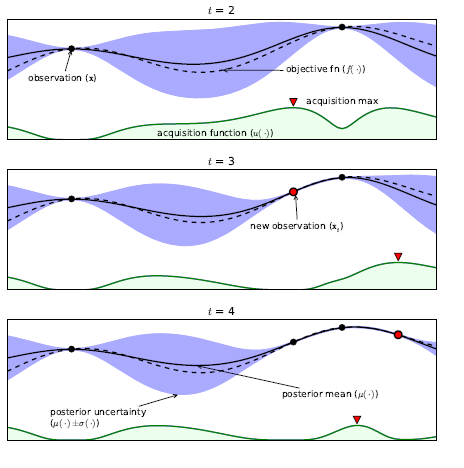
\includegraphics[width=.5\textwidth]{overview_1}
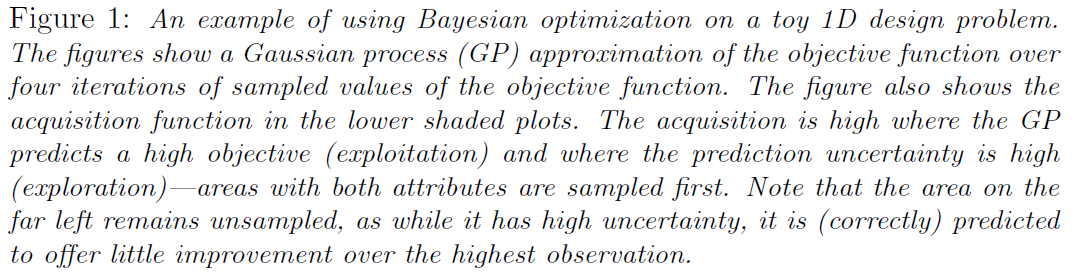
\includegraphics[width=.5\textwidth]{overview_2}
\end{center}
\end{frame}

%%%
\section{A Few Elements of Bayesian Optimization[5]}

%%
\subsection{Priors}
\begin{frame}{Priors}
\begin{itemize}
\item
We are to use Gaussian(normal) distribution for the prior, where we introduce the notion of \emph{Gaussian process}.
\item
The collection \(\{X_t:t\ge0\}\) of random variables \(X_t\) where \(t\) is indexed in a continuous domain is called the \alert{random process}.
\item
\alert{Gaussian process} is a kind of random process, where each of the \(X_t\) for \(t\ge0\) is distributed normally.
\end{itemize}
\end{frame}

%%
\begin{frame}{Priors}
\begin{itemize}
\item
We are to approxiamte the function \(f\).
\item
For each \(x\in A\), the value \(f(x)\) is not determined.
So we may think of \(f(x)\) as a random variable.
That is, we may think of \(\{f(x)|x\in A\}\) as a collection of random variable in a continuous domain \(A\).
\item
Assuming \(f(x)\) is distributed normally, we need only to specify its mean \(m(x)\) for each \(x\in A\) and covariance \(k(x,x')\) for each \(x,x'\in A\).
We write
\[f(x)\sim \mathcal G\mathcal P(m(x),k(x,x')).\]
\end{itemize}
\end{frame}

%%
\begin{frame}{Priors}
\begin{itemize}
\item
Still, the function \(m\) and \(k\) is not specified yet.
\item
For convenience, let \(m\) be a zero function;
\[m(x)=0.\quad(x\in A)\]
\item
We may choose \(k\) quite arbitrarily.
But the most popular choice is to use squared exponential function;
\[k(x_i,x_j)=\exp\left(-\frac12||x_i-x_j||^2\right).\]
\item
Note that the value \(k(x_i,x_j)\) converges to 1 as \((x_i-x_j)\) approaches to 0.
\end{itemize}
\end{frame}

%%
\subsection{Covariance Function}
\begin{frame}{Covariance Function}
\begin{itemize}
\item
The (popular) kernel function we have defined is quite a naive one.
We add a \alert{hyperparameter} \(\theta\) so that
\[k(x_i,x_j)=\exp\left(-\frac1{2\theta}||x_i-x_j||^2\right).\]
\item
For anisotropic models, we may set
\[k(x_i,x_j)=\exp\left(-\frac12(x_i-x_j)^T\text{diag}(\theta)^{-2}(x_i-x_j)\right),\]
where \(\text{diag}\) stands for a diagonal matrix of a vector \(\theta\).
\end{itemize}
\end{frame}

%%
\begin{frame}{Covariance Function}
\begin{itemize}
\item
Another important kernel for Bayesian Optimization is the Matérn kernel (Matérn, 1960 ; Stein, 1999)
\item
It incorporates a smoothness parameter \(\zeta\) to permit great flexibility in modelling functions:
\[k(x_i,x_j)=\frac1{2^{\zeta-1}\Gamma(\zeta)}\left(2\sqrt\zeta||x_i-x_j||\right)^\zeta H_\zeta\left(2\sqrt\zeta ||x_i-x_j||\right),\]
where \(\Gamma(\cdot)\) is the gamma function and \(H_\zeta(\cdot)\) is the Bessel function of order \(\zeta\).
\end{itemize}
\end{frame}


%%
\subsection{Acquisition Function}
\begin{frame}{Acquisition Function}
\begin{itemize}
\item
The acquisition function plays a role of guiding the search for the optimum.
\item
It is defined so that high acquisition is related to \emph{potentially} high values of the objective function \(f\).
\item
Denote \(u\) by the acquisition function.
\item
At timestep \(t\), we need to sample another point \(x_{t+1}\) from the domain.
We choose \(x_{t+1}\) as
\[x_{t+1}=\text{argmax}_{x\in A}u(x|D).\]
%By maximizing the acquisition funciton, we can choose the next point at which to evaluate the function.
\item
There are several kinds of acquisition functions, which we'll illustrate without deep explanation.
\end{itemize}
\end{frame}

%
\begin{frame}{Acquisition Function : PI}
%\begin{frame}{Probability of Improvement}
\begin{itemize}
\item
(Kushner, 1964) suggested maximizing \emph{probability of improvement} over the incumbent \(f(x^+)\) where
\[x^+=\text{argmax}_{1\le i\le t}f(x_i),\]
so that
\begin{align*}
\text{PI}(x)
&=P(f(x)\ge f(x^+))\\
&=\Phi\left(\frac{\mu(x)-f(x^+)}{\sigma(x)}\right).
\end{align*}
Here, \(\Phi\) stands for the normal cumulative distribution function.
\item
Kushner's approach is a natural, but greedy one.
It pursuits exploitation without exploration.
\end{itemize}
\end{frame}

%
\begin{frame}{Acquisition Function : EI}
\begin{itemize}
\item
More satisfing alternative acquisition function is the one which considers not only the probability of improvement, but also the magnitude of the improvement a point can potentially yield.
\item
(Močkus, 1978) Let \(I\) be a function (called \emph{improvement function}) defined by
\[I(x)=\max\{0,f_{t+1}(x)-f(x^+)\}.\]
Define the new point \(x\) at which we sample, by
\[x=\text{argmax}_x\mathbb E\left(\max\{0,f_{t+1}(x)-f(x^+)\}|D_t\right).\]
\end{itemize}
\end{frame}

%
\begin{frame}{Acquisition Function : Generalized EI}
\begin{itemize}
\item
EI, explained so far, can be evaluated analytically(Močkus, 1978 ; Jones, 1998) as follows;
\begin{center}
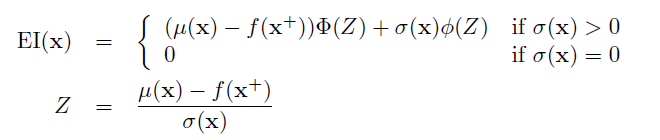
\includegraphics[width=.7\textwidth]{analytic_form_1}
\end{center}
\item
(Lizotte, 2008) suggests new acquisition function that enables us to trade off between exploration and exploitation
He adopted a parameter \(\xi\ge0\) such that
\begin{center}
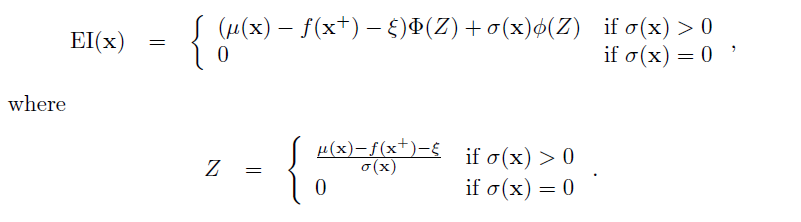
\includegraphics[width=.7\textwidth]{analytic_form_2}
\end{center}
\end{itemize}
\end{frame}



%
\frame{Thank you}
\end{document}
